\documentclass[a4paper, 12pt]{report}

% la lunghezza della sequenza di ../ dipende dalla profondita' della cartella
% in cui viene inserito il verbale rispetto alla cartella che contiene le 
% immagini.

\usepackage{charter}
\usepackage{makeidx}
\usepackage{fancyhdr}
\usepackage{hyperref}
\usepackage[utf8]{inputenc}
\usepackage{graphicx}
\usepackage[left=2cm, right=2cm]{geometry}
\usepackage{latexsym}
\usepackage{amsmath, amsthm, amssymb}
\usepackage{rotating}


\begin{titlepage}
\title{Secondo incontro con il committente\\Verbale 02/11/2009}
\date{ \\Firenze \\\begin{figure}[h] \centering 
\includegraphics[width=0.2\textwidth]{../../../../images/logokiwi.png} \end{figure} }
\end{titlepage}

\pagestyle{fancy}

\begin{document}

\maketitle

\newpage

\section*{Approvazione, redazione, lista distribuzione}
\begin{table}[h!]
  \begin{center}
    \begin{tabular}{| l | l | p{60mm} |}
    \hline
    \textbf{approvato da} & \textbf{il giorno} & \textbf{firma} \\
	\hline    
	Marco Tinacci & 07/11/2009 &  \\
    \hline
    \end{tabular}
  \end{center}
\end{table}

\begin{table}[h!]
  \begin{center}
    \begin{tabular}{| l | l | p{60mm} |}
    \hline
    \textbf{redatto da} & \textbf{il giorno} & \textbf{firma} \\
	\hline    
	Daniele Poggi & 03/11/2009 &  \\
    \hline
    \end{tabular}
  \end{center}
\end{table}

\begin{table}[h!]
  \begin{center}
    \begin{tabular}{| l | l | p{60mm} |}
    \hline
    \textbf{hanno partecipato} & \textbf{il giorno} & \textbf{firma} \\
	\hline    
	Francesco Calabri & 07/11/2009 &  \\
    \hline
	Manuele Paulantonio & 07/11/2009 &  \\
    \hline
	Daniele Poggi & 07/11/2009 &  \\
    \hline
	Massimo Nocentini & 07/11/2009 &  \\
    \hline
	Niccol\'o Rogai & 07/11/2009 &  \\
    \hline
	Marco Tinacci & 07/11/2009 &  \\
    \hline
    \end{tabular}
  \end{center}
\end{table}

\newpage

\section*{Ora e sede}
13.30 Viale Morgagni

\section*{Invitati e presenti}
Committente PMango e Fornitori

\section*{Ordine del giorno}
\begin{itemize}
  \item Rappresentazione dipendenze sui Gantt e nei TaskNetworks
  \item Rappresentazione del cammino Critical Path e del Time Gap 
\end{itemize}

\section*{Discussione}
\begin{itemize}
  \item Le dipendenze sono da rappresentare solo nel Gantt (opzione dell'utente) e nei TaskNetworks.
	 Ogni dipendenza va applicata sui task di base e non su quelli composti che in ogni caso
	 la ereditano.
	 Per la rappresentazione delle dipendenze in task composti è stato adottato la seguente simbologia:
	 \begin{figure}[h!] 
				\centering 
				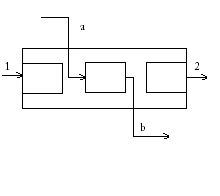
\includegraphics[width=0.4\textwidth]{img1.png} 
				\caption{dipendenze}
				\label{fig:dipendenze}			
			\end{figure}
	 le frecce 1 e 2 si applicano nel caso in cui si fa riferimento rispettivamente all'inizio o alla fine
	 del task composto, nel caso in cui invece una dipendenza fa riferimento ad un task "nel mezzo" si utilizza "a" e "b"
	 cercando di centrarle nel riquadro.
	 Nel caso di maggior confluenza di frecce si adotta la seguente rappresentazione
	 \begin{figure}[h!] 
				\centering 
				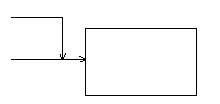
\includegraphics[width=0.3\textwidth]{img2.png} 
				\caption{schema}
				\label{fig:schema}			
			\end{figure}
	 In ultimo nelle tasknetworks non si disegnano i padri se sono presenti i figli.
	 Se i contenuti del padre sono aperti si disegna solo i contenuti altrimenti si disegna solo il padre con una notazione 
	 + che specifica che sono presenti dei sottotask.

  \item Nei tasknetworks si deve disegnare il critical path, evidenziandolo con delle linee più spesse.
	 In nessun caso utilizzare colori, sono preferiti il bianco e nero e la scala di grigi.	 
 
\end{itemize}
 	 
\section*{Varie e eventuali}
Domande del team:
\begin{itemize}
  \item Nel caso in cui vi siano discordanze temporali in una WBS o in una TaskNetworks come si possono rappresentare?
   Si utilizza un "delta" per quelle lievi "delta!" per quelle gravi.  
  \item Come si possono distinguere i casi lievi e quelli gravi? 
	 Le cause lievi sono tutte quelle che non procedono secondo l'ordine programmato ma che comunque non influiscono
	 negativamente, mentre quelle gravi sono tutte quelle che eccedano il loro tempo massimo, costano di più ...
  \item Può servire una funzione di Zoom nel caso di una rappresentazione grafica?
	 Sarebbe interessante e utile avere a disposizione dei comandi che permettono all'utente di decidere la risoluzione
	 dell'immagine finale, nel caso da rappresentare in un'altra finestra. Comoda sarebbe la possibilità per l'utente
	 di specificare una risoluzione e di poterla poi utilizzare tutte le volte che usa il programma.   
\end{itemize}

\section*{Chiusura della riunione}
Riunione chiusa alle 15:30

\end{document}